% Chapter Template

\chapter{Descriptive Statistics} % Main chapter title

\label{Chapter3} % Change X to a consecutive number; for referencing this chapter elsewhere, use \cref{ChapterX}

%----------------------------------------------------------------------------------------
%	SECTION 1
%----------------------------------------------------------------------------------------


The number of different possible hands is:
\[ N = {36\choose 9}  = 94'\,143'\,280 \]
Using all combinations in a reasonable time for training will not be feasible because the computational cost can not be satisfied with the hardware at hand.
1'\,000'\,000 hands were generated to be used for the descriptive statistics. \\

As expected, the cards are completely random, and no pattern can be seen. (Figure \ref{fig:scatter_matrix})

\begin{figure}[ht!]
    \centering
    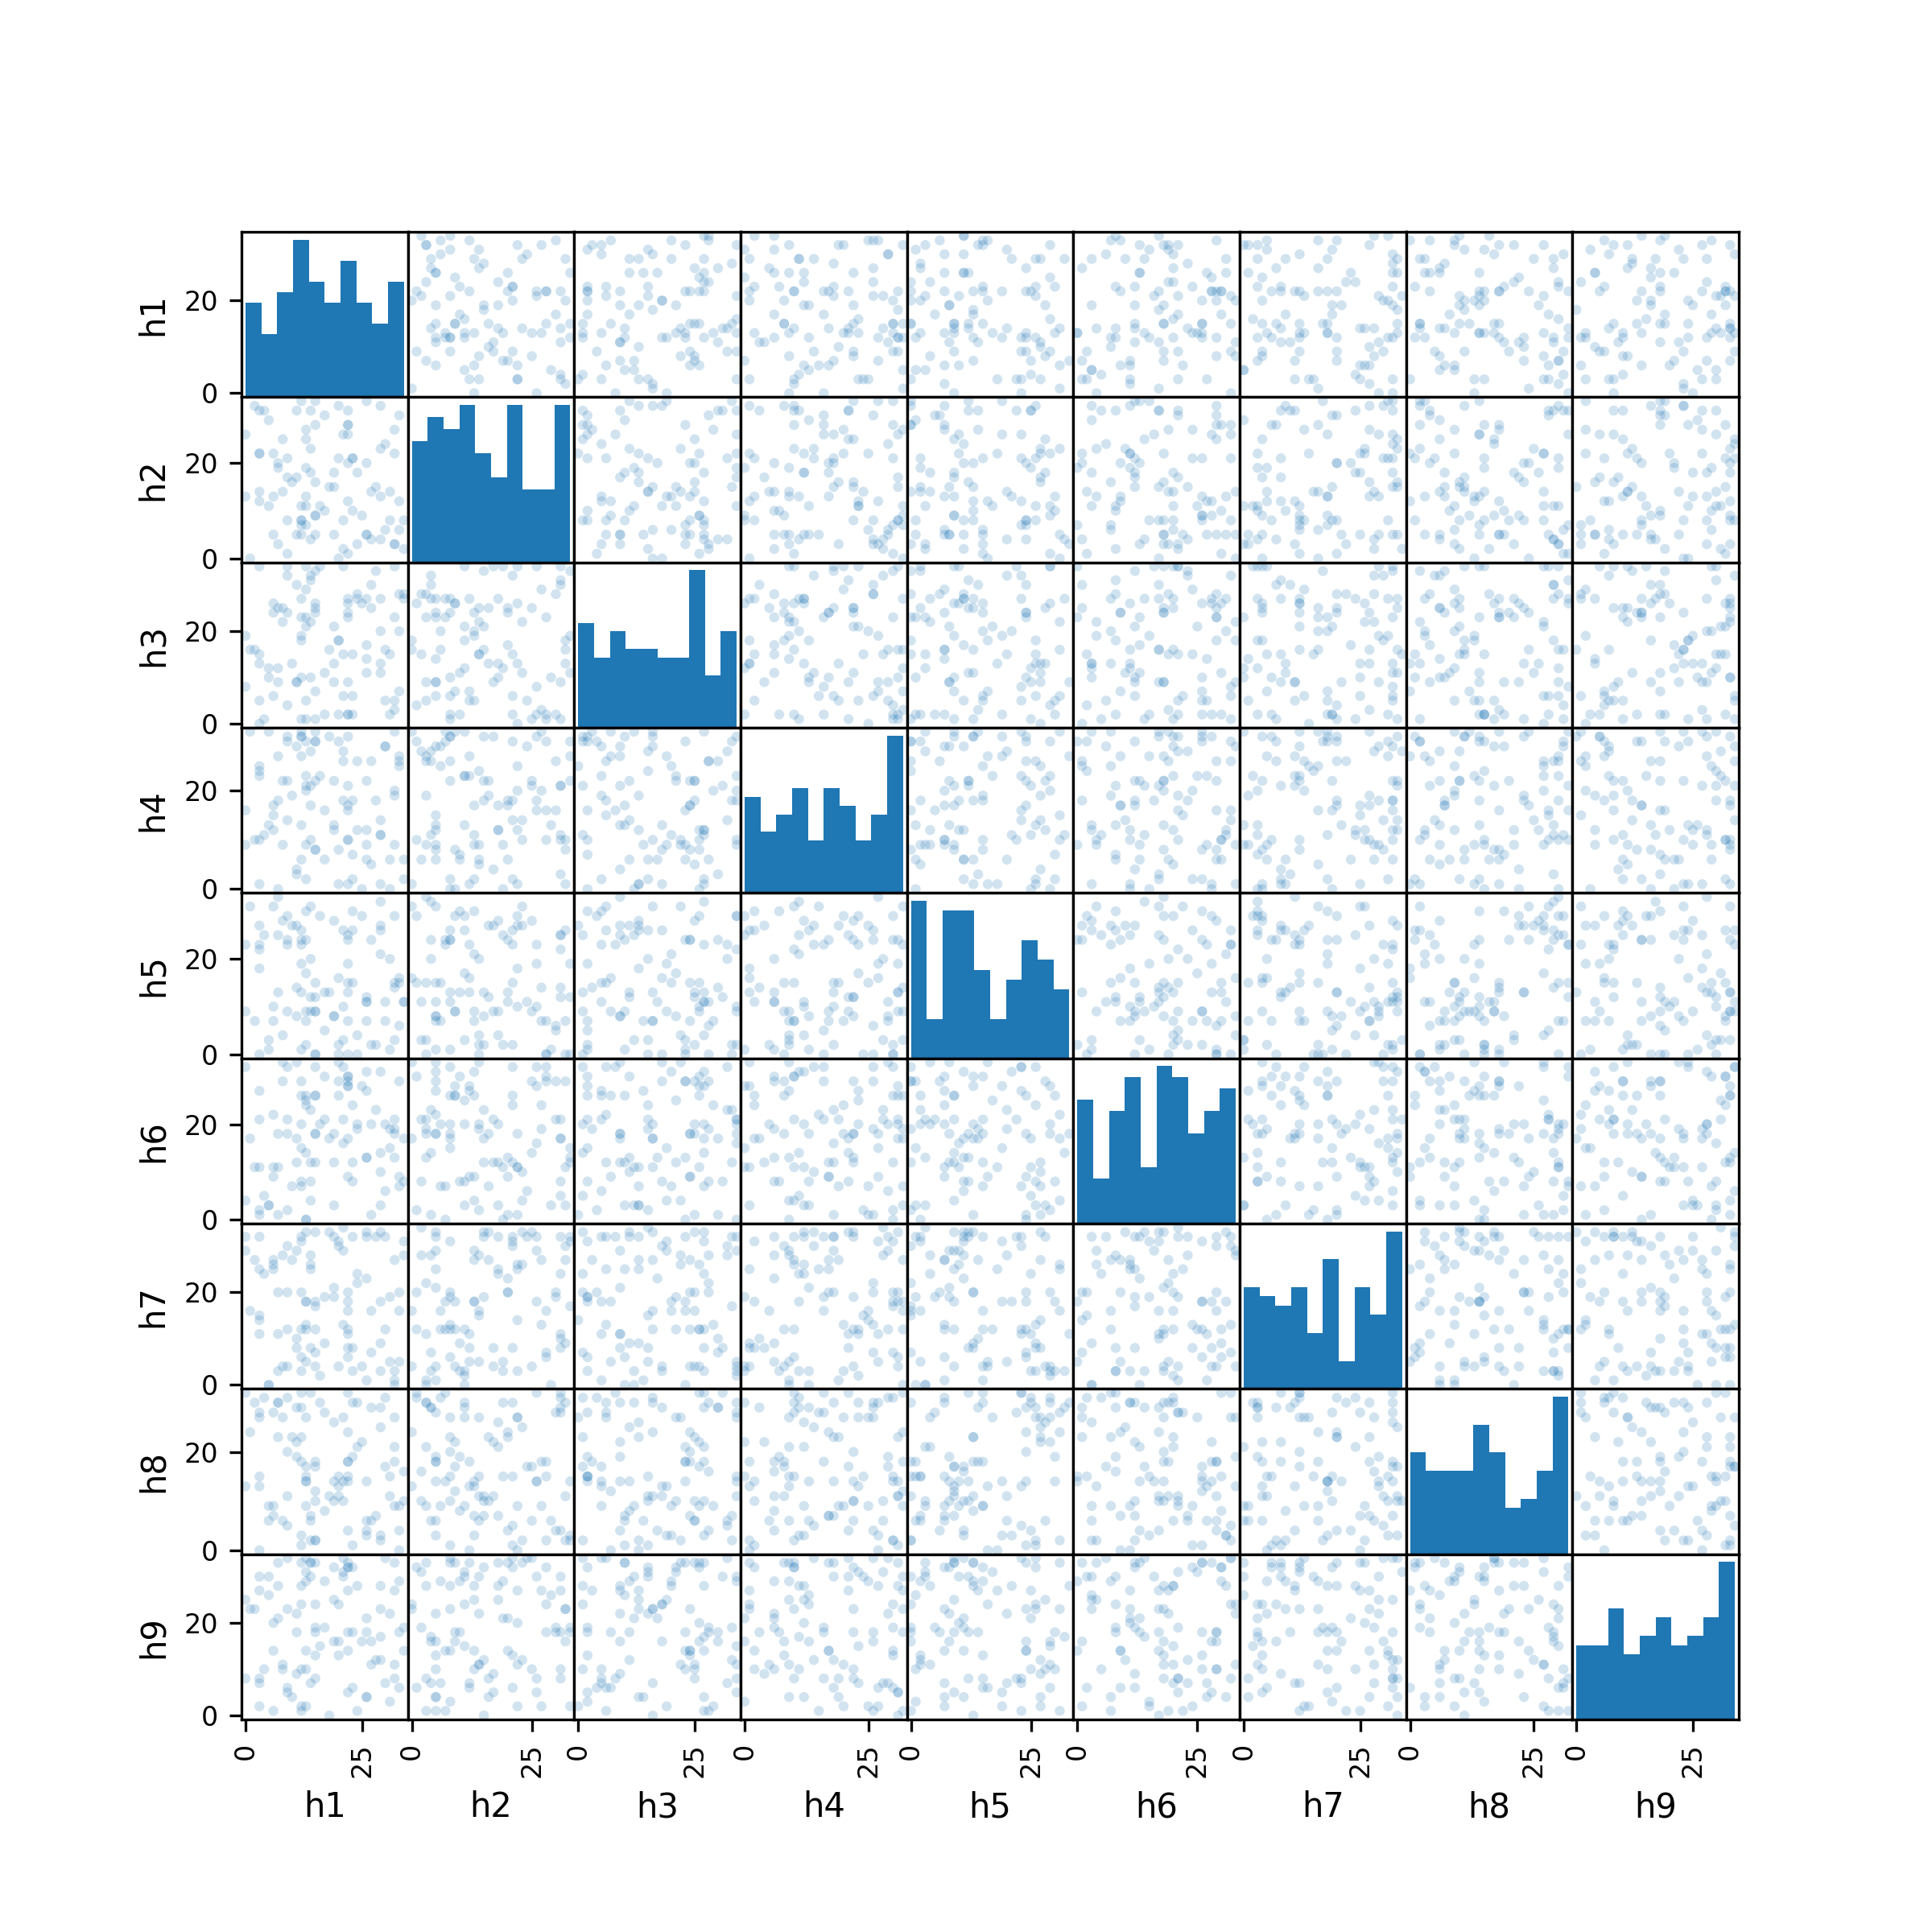
\includegraphics[width=0.9\textwidth]{Figures/scatter_matrix_hand}
    \decoRule
    \caption[Scatter Matrix of 1'\,000'\,000 hands]{Scatter Matrix of 1'\,000'\,000 hands}
    \label{fig:scatter_matrix}
\end{figure} 

